\documentclass{trkut}% Reaalkooli vormistus. Muidu "report" või "article".
\usepackage[style=trkut]{biblatex}% Kasutatud kirjanduse genereerimine
\usepackage{mleftright, braket}
\addbibresource{viited_kaarel_kivisalu.bib}% Viidete info fail
\defbibheading{bibliography}{\addchap{#1}}% Lisame kasutatud materjalid sisukorda

\pealkiri{Gravitatsiooni mõju kera soojusmahtuvusele}
\autor{Kaarel Kivisalu}
\klass{11. a}
\juhendaja{prof Jaan Kalda \\ õp Toomas Reimann}
\toggletrue{mitujuhendajat}% Uncomment kui on mitu juhendajat

\DeclareMathOperator{\tr}{tr}
\DeclareMathOperator{\erf}{erf}
\NewDocumentCommand{\op}{o m}{\IfNoValueTF{#1}{\hat{#2}}{\hat{#2}^{#1}}}
\renewcommand\bra[1]{{\langle{#1}|}}
\renewcommand\ket[1]{{|{#1}\rangle}}
\renewcommand\Bra[1]{\mleft\langle#1\mright|}
\renewcommand\Ket[1]{\mleft|#1\mright\rangle}
\renewcommand\braket[1]{\langle{#1}\rangle}
\reversemarginpar

\begin{document}
\maketitle% Tiitelleht
\tableofcontents% Sisukord
\addchap{Sissejuhatus}
\nummerdame% See käsk peab olema õigeks nummerdamiseks kohe peale sissejuhatust
I rahvusvahelisel füüsikaolümpiaadil 1967. aastal oli järgnev probleem \cite{ipho67}:

\textit{Kaks homogeenset ühesugust kera on sama algtemperatuuriga. Üks kera on liikumatult horisontaalse tasandil, teine ripub niidi küljes. Mõlemale kerale antakse võrdne soojushulk. Kas kerade lõpptemperatuur on sama või mitte. Soojuskadudega mitte arvestada.}

Käesolevas töös uuritakse konkreetsete potentsiaalide korral konstantse gravitatsioonvälja mõju kera soojusmahtuvusele.
Konstantse gravitatsioonivälja potentsiaal on lineaarne.
Vaadatakse soojusmahtuvuse erinevust juhtudel, kui on ainult kera potentsiaal ja kera potentsiaalile on lisatud lineaarne gravitatsioonivälja potentsiaal.

Töös on analüüsitud kuuppolünoompotentsiaali häirituse meetodil ja kahest lineaarsest funktsioonist koosnevat potentsiaali kvaasi-klassikaliselt. Samuti on näidatud, et osade potentsiaalide korral ei mõjuta gravitatsioon soojusmahtuvust.

Varem on uuritud gravitatsiooni mõju metallkera soojusmahtuvusele üldjuhul.
Leiti üldine seos soojusmahtuvuse, temperatuuri, gravitatsioonivälja tugevuse ja lineaarse soojuspaisumisteguri vahel.
Saadud tulemust on eksperimentaalselt väga raske kinnitada, kuna gravitatsiooni mõju on väga väike. Konkreetsete potentsiaalide läbivaatamine tõstaks ka varem leitud mudeli usaldusväärsust.

Uurimistöö hüpotees on, et sõltuvalt potentsiaalist võib gravitatsioon nii tõsta kui ka langetada keha soojusmahtuvust.
\addchap{Tähiste loetelu}
\chapter{Teoreetiline osa}

\section{Tavapärane lahendus}

Tavapärane lahendus põhineb soojuspaisumisega seotud erinevustel. Kerale $A$ soojust andes see paisub ja selle massikese tõuseb. Järelikult peab osa kerale A antavast soojushulgast kuluma kera massikeskme gravitatsioonilise potentsiaalse energia tõstmiseks ja lõpptemperatuur on madalam algsest. Vastupidiselt, kera $B$ massikese langeb soojuspaisumise tõttu ja energiat saadakse juurde, järelikult on kera $B$ lõpptemperatuur kõrgem.

Pannakse ka kirja tavapärasele lahendusele vastavad valemid. Olgu kerade soojusmahtuvus $C_0$ gravitatsioonivälja puudumisel. Tavapärase lahenduse korrale, kui kera A soojendatakse, siis selle massikese tõused $dR=\alpha R \, dT$ võrra, kus $dT$ on temperatuuri tõus, $\alpha$ on soojuspaisumistegur ja $R$ on kera raadius. Kera saab potentsiaalse energia $d\Phi = mg \, dR$, kus $m$ on keha mass ja $g$ on raskuskiirendus. Järelikult, kui soojushulk \(\delta Q\) antakse süsteemile, siis saadakse, et
\begin{equation}
    \delta Q = C_0 \, dT + mg \, dR = C_0 \, dT + mg\alpha R \, dT = (C_0 +  mg\alpha R) dT.
\end{equation}
See on ekvivalentne väitega, et kera \(A\) soojusmahtuvus on:
\begin{equation}
    C_A = C_0 + mg\alpha R.
\end{equation}
Analgoselt saame, et kera \(B\) soojusmahtuvus on
\begin{equation}
    C_B = C_0 - mg\alpha R.
\end{equation}
Enamiku materjalide jaoks on \(\alpha > 0\), millest tulenevalt \(C_A>C_B\). Järelikult on tavapärase lahenduse kohaselt kera \(A\) lõpptemperatuur madalam kera \(B\) lõpptemperatuurist.

\section{Tavapärane lahendus ja selle termodünaamika II seaduse rikkumine}

Tavapärases lahenduses kaudselt eeldatakse, et keha siseenergia \(U\) ja raadius \(R\) sõltuvad ainult temperatuurist \(T\), mitte aga raskuskiirendusest \(g\). Vaadeltakse järgnevat tsüklit: pall asub horisontaalsel külmal tasandil temperatuuriga \(T_1\); pall ühendatakse soojema reservuaariga, mille temperatuur \(T_2=T_1+dT>T_1\); pall riputatakse nööri külge ja horisontaalne tasand eemaldatakse; pall ühendatakse külma reservuaariga, mille temperatuur on \(T_1\). Selle protsessi kasutegur on tehtud töö ja neeldunud soojuse suhe ning avaldub kujul \cite{palma15}
\begin{equation}
    \eta = \frac{2mg\alpha R}{C_0+mg\alpha R}.
\end{equation}
Kasutegur \(\eta\) ei sõltu \(dT\) suurusest. Termodünaamika teist seadus saab sõastada järgnevalt: iga tsükkel, mis töötab ainult temperatuuride \(T_1\) ja \(T_2\) juures ei saa olla efektiivsem Carnot' tsüklist, mis töötab samade temperatuuride juures. Carnot' tsükli efektiivsus on
\begin{equation}
    \eta_{Carnot'} = \frac{dT}{T_2}
\end{equation}
Järelikult, kui \(dT\) on piisavalt väike, siis on palliga tsükli kasutegur suurem Carnot' tsükli kasutegurist. Teisisõnu rikub tavapärane lahendus termodünaamika II seadust.
\begin{figure}[h]
    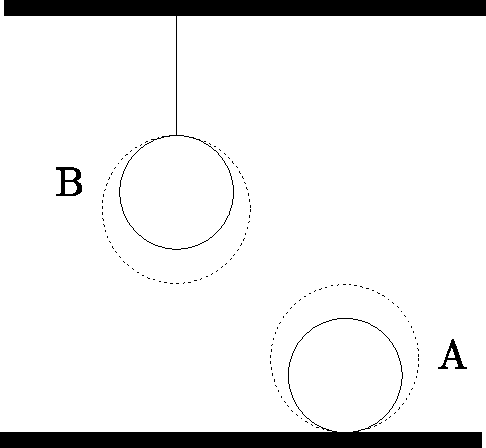
\includegraphics[width=0.5\textwidth]{joonis1.pdf}
    \caption{Probleemi ülesehitus}
    \allikas{\protect\cite{palma15}}
    \label{iphojoonis}% Selle järgi viidatakse, see rida peab olema pärast \caption
\end{figure}

\section{Statistiline mehaanika}

Kasutades statistilise mehaanika meetodeid on võimalik leida kera soojusmahtuvuse sõltuvus gravitatsioonist \parencite[test]{palma15}:
\begin{equation}
    \frac{\partial C(g,T)}{\partial g} = -mTY \left( \alpha^2 + \frac{\partial \alpha}{\partial T} \right),
\end{equation}
kus \(C\) on soojusmahtuvus, \(g\) on raskuskiirenuds, \(m\) on kera mass, \(T\) on kera temperatuur, \(Y\) on massikeskme kõrgus, \(\alpha\) on lineaarne soojuspaisumistegur.

%\section{Schrödingeri võrrand}
%
%Ajast sõltumatu Schrödingeri võrrand ühes dimensioonis avaldub kujul \cite{griffiths05}
%\begin{equation}
%    \op{H} \Psi = E \Psi,
%\end{equation}
%kus \(E\) on süsteemi koguenergia ja
%\begin{equation}
%    \op{H}=-\frac{\hbar^2}{2m}\frac{d^2}{dx^2}+V(x).
%\end{equation}

\section{Energiatasemed ja soojusmahtuvus}
Kvantmehaanilises statistilises mehaanikas on mugav kasutada tihedusmaatriksit (ingl \textit{density matrix}) $\op{\rho}$ kvantmehaanilise operaatori ooteväärtuse (ingl \textit{expectation value}) leidmiseks.
Tihedusmaatriks on defineeritud järgnevalt \parencite[172]{kardar07}:
\begin{equation}
    \op{\rho}(t) \equiv \sum_j p_j \ket{\Psi_j(t)} \bra{\Psi_j(t)},
\end{equation}
kus $\sum_j p_j=1$, $p_j > 0$ ja $\ket{\Psi_j}$ on puhas kvantolek (ingl \textit{pure quantum state}).
See kujutab segakvantolekut (ingl \textit{mixed quantum state}), kus tõenäosusega $p_j$ on süsteem puhtas kvantolekus $\ket{\Psi_j}$.
Selles formalismis avaldub kvantmehaanilise operaatori ooteväärtuse ansambli keskväärtus järgnevalt \parencite[172]{kardar07}:
\begin{equation}
    \overline{\braket{\op{O}}}=\tr(\op{\rho}\op{O}),
    \label{ootev}
\end{equation}
kus jälg (ingl \textit{trace}) $\tr(\op{A}) \equiv \sum_n \braket{n|\op{A}|n}$\footnote{\url{http://en.citizendium.org/wiki/Trace_\%28mathematics\%29} lõputu dimensioon converges} \parencite{viide}.
Kanoonilise ansambli\footnote{Ansambel, kus süsteem on soojuslikus tasakaalus fikseeritud temperatuuriga reservuaariga.} jaoks, mis on kvantmehaaniline ja diskreetne, avaldub kanooniline tihedusmaatriks järgnevalt \parencite[174]{kardar07}:
\begin{equation}
    \op{\rho}(\beta) = \frac{e^{-\beta \op{H}}}{Z(\beta)},
    \label{tihm}
\end{equation}
kus $\beta \equiv 1/k_B T$, kus $T$ on temperatuur ja $k_B$ on Boltzmanni konstant,
Kuna $\bra{\Psi_j}$ on normaliseeritud, siis
\begin{equation}
    \braket{1}=\tr(\op{\rho})=\sum_n \braket{n|\op{\rho}|n}=\sum_{n, j} p_j |\braket{n| \Psi_j}|^2=\sum_j p_j=1.
    \label{tihnorm}
\end{equation}
Võrranditest \eqref{tihm} ja \eqref{tihnorm} ning omadusest $\tr(c\op{A})=c\tr(\op{A})$ saadakse kvantmehaaniline statistiline summa $Z$, mis avaldub kujul
\begin{equation}
    Z=\tr(e^{-\beta \op{H}})=\sum_n e^{-\beta \op{H}}.
    \label{part}
\end{equation}
Kasutades võrrandeid \eqref{ootev}, \eqref{tihm} ja \eqref{part} saadakse hamiltoniaani $\op{H}$ keskmine ooteväärtus
\begin{equation}
    \overline{\braket{\op{H}}}=\tr(\op{\rho}\op{H})=\frac{\tr{\op{H}e^{-\beta \op{H}}}}{Z}= -\frac{\partial \ln Z}{\partial \beta}.
    \label{keskham}
\end{equation}
Hamiltoniaani keskmist ooteväärtust võib mõista kui süsteemi energait. Kuna ollakse huvitatud temperatuuri muutusel kui süsteemile antakse mingi enerigiahulk, siis on kasulik defineerida soojusmahtuvus kui
\begin{equation}
    C = \frac{\partial \overline{\braket{\op{H}}}}{\partial T}.
    \label{soojuham}
\end{equation}
Kombineerides võrrandeid \eqref{keskham} ja \eqref{soojuham} saadakse, et
\begin{equation}
    C = k T^2 \frac{\partial^2 \ln Z}{\partial \beta^2}
    \label{mahtuvus}
\end{equation}


\section{Kvaasi-klassikaline lähendus}

Schrödingeri võrrandi
\begin{equation}
    -\frac{\hbar^2}{2m}\frac{d^2\psi}{dx^2}+V(x)\psi=E\psi
\end{equation}
saab ümber kirjutada järgnevalt:
\begin{equation}
    \frac{d^2 \psi}{dx^2}= - \frac{p^2}{\hbar^2}\psi,
\end{equation}
kus
\begin{equation}
    p(x) \equiv \sqrt{2m[E-V(x)]}
\end{equation}
on klassikaline valem osakese impulsi jaoks koguenergiaga $E$ ja potentsiaalse energiaga $V(x)$.
Piirkonnas, kus $E>V(x)$, on $p(x)$ reaalne.
Seda piirkonda kutsutakse \enquote{klassikaliseks}, kuna klasskikaliselt on osake piiratud selles piirkonnas.
Üldiselt on $\psi$ kompleksfunktsioon, mida saab avaldada klassikalises piirkonnas amplituudi $A(x)$ ja faasi $\phi(x)$ kaudu, mis mõlemad on reaalsed \parencite[316]{griffiths05}:
\begin{equation}
    \psi(x)=A(x)e^{i\phi(x)}.
\end{equation}
\marginpar{Kas oleks vaja tuletuskäiku?}Eeldades, et amplituud $A$ muutub aeglaselt\footnote{Täpsemalt eeldatakse, et $A''/A\ll(\phi ')^2$ ja $A''/A\ll p^2/\hbar^2$.}, avaldub lainefunktsioon klassikalises piirkonnas kujul \parencite[316-318]{griffiths05}
\begin{equation}
    \psi = \frac{C_1}{\sqrt{p(x)}}\exp\left(\frac{i}{\hbar}\int p(x)\, dx\right) +\frac{C_2}{\sqrt{p(x)}}\exp\left(-\frac{i}{\hbar}\int p(x)\, dx\right),
    \label{eq:kvaasik1}
\end{equation}
kus $C_1$ ja $C_2$ on kompleksarvulised konstandid.
Valemi \eqref{eq:kvaasik1} saab ka kirja panna kujul \parencite[446]{shankar94}
\begin{equation}
    \psi(x)=\frac{A}{\sqrt{p(x)}} \cos \left[ \frac{1}{\hbar}\int p(x)\, dx + B \right],
    \label{eq:kvaasik2}
\end{equation}
kus $A$ ja $B$ on reaalsed parameetrid.
Kahjuks ei kehti \eqref{eq:kvaasik2} kui $E \approx V(x)$, kuna $\sqrt{p(x)} \to 0$. Olgu $V(x_1)=V(x_2)=E$, $x_1<x_2$ ja lõigul $(x_1, x_2)$ on $V(x)<E$.
\marginpar{Kas oleks vaja tuletuskäiku?}On siiski võimalik vaadeldes lainefunktsiooni $x_1$ lähedal näidata, et lõigul $(x_1, x_2)$ on lainefunktsioon järgmine \parencite[167-170]{landau05}:
\begin{equation}
    \psi(x)=\frac{A}{\sqrt{p(x)}} \cos \left[ \frac{1}{\hbar}\int_{x_1}^{x} p(x)\, dx - \frac{\pi}{4} \right],
\end{equation}
kui $x_2$ lähedal on lainefunktsioon
\begin{equation}
    \psi(x)=\frac{A'}{\sqrt{p(x)}} \cos \left[ \frac{1}{\hbar}\int_{x_2}^{x} p(x)\, dx + \frac{\pi}{4} \right].
\end{equation}
Selleks, et need kaks lahendit ühtiksid, peavad $A$ ja $A'$ olema sama magnituudiga ja koosinuste faaside vahe peab olema $\pi$ kordne \parencite[446]{shankar94}:
\begin{equation}
    \frac{1}{\hbar}\int_{x_1}^{x} p(x)\, dx - \frac{1}{\hbar}\int_{x_2}^{x} p(x)\, dx - \frac{\pi}{2} = n\pi
\end{equation}
või
\begin{equation}
    \int_{x_1}^{x_2} p(x)\, dx =\left(n+\frac{1}{2}\right)\pi \hbar.
\end{equation}



\section{Ajast sõltumatu häiritusteooria}

Schrödingeri võrrandit täpselt lahendada on võimalik ainult lihtsamatel juhtudel, keerulisemate juhtude jaoks on vaja teha lähendusi.
Ajast sõltumatu häiritusteooria (edaspidi häiritusteooria) on lähendusmeetod, mida saab rakendada järgnevas olukorras: teades lahendit hamiltoniaani $\op[0]{H}$ omaväärtusülesandele (ingl \textit{eigenvalue problem}), tahetakse leida lahendit $\op{H}=\op[0]{H}+\op[1]{H}$, kus $\op[1]{H}$ on suhteliselt väike võrreldes $\op[0]{H}$-ga.
Eeldatakse, et iga $\op[0]{H}$ kidumata omaketi (ingl \textit{eigenket}) $\Ket{n^0}$ omaväärtusega $E_n^0$ jaoks leidub $\op{H}$ kidumata omaket $\Ket{n}$ omaväärtusega $E_n$.
Siis eeldades, et $H$ omaketid ja omaväärtused võib kirja panna häiritusseerias \parencite[451]{shankar94}:
\begin{align}
    \Ket{n}&=\Ket{n^0}+\Ket{n^1}+\Ket{n^2}+... \\
    E_n&=E_n^0+E_n^1+E_n^2+...
\end{align}
Iga liikme ülaindeks $k$ näitab millise $\op[1]{H}$ astmega eeldatakse, et iga liige on võrdeline.
Selleks, et leida liikmeid $\Ket{n}$ ja $E_n$ arenduses, alustatakse omaväärtusvõrrandiga \parencite[451-452]{shankar94}:
\begin{equation}
    \op{H}\ket{n}=E_n\ket{n}
\end{equation}
või
\begin{equation}
    (\op[0]{H} + \op[1]{H})(\ket{n^0}+\ket{n^1}+...)=(E_n^0+E_n^1+...) (\ket{n^0}+\ket{n^1}+...).
    \label{terms}
\end{equation}
Vaadates võrrandis \eqref{terms} nullindat järku liikmeid saadakse võrrand
\begin{equation}
    \op[0]{H}\ket{n^0}=E_n^0\ket{n^0}.
\end{equation}
Eelduse järgi on see võrrand lahendatud ja omaket $\Ket{n^0}$ ja omaväärtused $E_n^0$ on teada. Vaadates võrrandis \eqref{terms} esimest järku liikmeid saadakse võrrand
\begin{equation}
    \op[0]{H}\ket{n^1} + \op[1]{H}\ket{n^0} = E_n^0\ket{n^1} + E_n^1\ket{n^0}.
    \label{terms1}
\end{equation}
Korrutades võrrandi \eqref{terms1} mõlemad pooled $\bra{n^0}$-ga ning kasutades omadusi $\bra{n^0}\op[0]{H}=\bra{n^0}E_n^0$ ja $\braket{n^0|n^0}=1$ saadakse, et
\begin{equation}
    E_n^1=\braket{n^0|\op[1]{H}|n^0}.
    \label{parand1}
\end{equation}
\marginpar{Kas oleks vaja tuletuskäiku?}Sarnaselt on võimalik saada teist järku parand energiale, mis avaldub kujul \parencite[451-453]{shankar94}:
\begin{equation}
    E_n^2=\sum_{m \neq n} \frac{|\braket{n^0|\op[1]{H}|m^0}|^2}{E_n^0-E_m^0}
    \label{parand2}
\end{equation}

%Häirituse teooria diskreetse spektrumi jaoks saab formuleerida järgnevalt. Eeldatakse, et on teada diskreetse spektri omaväärtused (ingl  \textit{eigenvalues}) \(E_0^{(0)}\) ja omafunktsioonid (ingl \textit{eigenfunctions}) \(\phi^0\) häitimata operaatori \(H_0\) jaoks, st et on teada võrrandi
%\begin{equation}
%    H_0 \psi=E_0 \psi
%\end{equation}
%täpsed lahendid. Soovitakse leida ligikaudseid lahendeid võrrandile
%\begin{equation}
%    \op{H} \psi=(H_0+V)\psi=E\psi,
%\end{equation}
%st ligikaudesd avaldised häiritud operaatori \(\op{H}\) omafunktsioonide \(\phi_n\) ja omaväärtuste \(E_n\) väärtused.\parencite{landau05}

\chapter{Praktiline osa}

Käesolevas osas leitakse konkreetsetele võimalikele kera potentsiaalidele vastavad soojusmahtuvuse sõltuvused gravitatsioonist, kus gravitatsiooni potentsiaal on võetud lineaarseks sõltuvalt ühest koordinaadist.
Kuigi tegelik kera potentsiaal on keeruline võib anda konkreetne potentsiaal küllaltki täpse lahendi.

\section{Tükiti lineaarne potentsiaal}
Vaadeldakse potentsiaali kujuga
\begin{equation}
    V(x)=\begin{cases}
        (-a+mg)x, & x<0,\\
        (b+mg)x, & x\ge0,
    \end{cases}
\end{equation}
kus $a$ ja $b$ on positiivsed reaalarvulised konstandid ning $-a+mg<0$ ja $b+mg>0$.
Kvaasi-klassikalises lähenduses saame leida vastava energiatasemed:
\begin{equation}
    \left( n+\frac{1}{2}\right)\pi \hbar = \int_{x_1}^{0} \sqrt{2m[E_n-(-a+mg)x]}\, dx + \int_{0}^{x_2} \sqrt{2m[E_n-(b+mg)x]} \, dx,
\end{equation}
kus \(n \in \{0, 1, 2, ...\}\), \(x_1=\frac{E_n}{-a+mg}\) ja \(x_2=\frac{E_n}{b+mg}\). Integreerides saadakse, et
\begin{align}
    \left(n+\frac{1}{2}\right)\pi \hbar &= \sqrt{2m}\left.\left[-\frac{2(E_n-(-a-mg)x)^\frac{2}{3}}{3(-a+mg)}\right]\right|^0_{x_1} + \sqrt{2m}\left.\left[-\frac{2(E_n-(b-mg)x)^\frac{2}{3}}{3(b+mg)}\right]\right|^{0}_{x_2} \notag \\
    &= -\frac{2\sqrt{2m}E_n^{\frac{3}{2}}}{3(-a+mg)}+\frac{2\sqrt{2m}E_n^{\frac{3}{2}}}{3(b+mg)}.
\end{align}
$E_n$ avaldades saadakse, et
\begin{equation}
    E_n =\left[\frac{3\pi}{2\sqrt{2}} \frac{\hbar}{\sqrt{m}} \frac{(-a+mg)(b+mg)}{a+b}\right]^{\frac{2}{3}} \left(n+\frac{1}{2}\right)^{\frac{2}{3}} . \label{tukene}
\end{equation}
Asendades võrrandisse \eqref{tukene} $c=\left[\frac{3\pi}{2\sqrt{2}} \frac{\hbar}{\sqrt{m}} \frac{(-a+mg)(b+mg)}{a+b}\right]^{\frac{2}{3}}$ avaldub statistiline summa järgnevalt:
\begin{equation}
    Z=\sum_{n=0}^{\infty} \exp \left( -\beta c \left(n+\frac{1}{2}\right)^\frac{2}{3} \right).
    \label{linsum}
\end{equation}
Kui $\beta c\ll 1$, siis saab summa asendada integraaliga ja $n+\frac{1}{2}\approx n$:
\begin{equation}
    Z \approx \int_0^\infty e^{-\beta c n^\frac{2}{3}} \, dn = \left.\left[ \frac{3\sqrt{\pi}  \erf{\left( {n}^\frac{1}{3} \sqrt{\beta c}\right)} }{4 (\beta c)^\frac{3}{2}}-\frac{3n^\frac{1}{3} e^{-\beta cn^\frac{2}{3}}}{2 \beta c }\right]\right|^{\infty}_{0} =\frac{3\sqrt{\pi}}{4(\beta c)^\frac{3}{2}} .
    \label{linpart}
\end{equation}
Võrrandist \eqref{mahtuvus} ja \eqref{linpart} saadakse, et
\begin{equation}
    C=kT^2 \frac{\partial^2}{\partial \beta^2} \ln \frac{3\sqrt{\pi}}{4(\beta c)^\frac{3}{2}}=-k_BT^2\frac{\partial}{\partial \beta} \frac{3}{2\beta}=\frac{3k_B}{2}
\end{equation}
See tähendab, et kõrgetel temperatuuridel ei sõltu süsteemi soojusmahtuvus temperatuurist.
Üldisemalt avaldub soojusmahtuvus võrranditest \eqref{mahtuvus} ja \eqref{linsum} järgnevalt:
\begin{align}
    C={}&kT^2 \frac{\partial^2}{\partial \beta^2} \ln Z \nonumber \\
    ={}&kT^2\frac{\partial}{\partial \beta}\frac{1}{Z} \frac{\partial Z}{\partial \beta} \nonumber \\
    ={}&kT^2\frac{\partial}{\partial \beta}\frac{1}{Z} \sum_{n=0}^{\infty} \frac{\partial}{\partial \beta} \exp \left( -\beta c \left(n+\frac{1}{2}\right)^\frac{2}{3} \right) \nonumber \\
    ={}&kT^2\frac{\partial}{\partial \beta} \frac{\sum_{n=0}^{\infty} -c\left(n+\frac{1}{2}\right)^\frac{2}{3} \exp \left( -\beta c \left(n+\frac{1}{2}\right)^\frac{2}{3} \right)}{\sum_{n=0}^{\infty} \exp \left( -\beta c \left(n+\frac{1}{2}\right)^\frac{2}{3} \right)} \nonumber \\
    \begin{split}\label{mahsum}
        ={}&kT^2 \frac{c^2 \sum_{n=0}^\infty \left( n+\frac{1}{2}\right)^\frac{4}{3} \exp \left( -c \left( n+\frac{1}{2} \right)^\frac{2}{3} \beta \right) }{\sum_{n=0}^\infty {{\exp}\left( -c {{\left( n+\frac{1}{2}\right) }^{\frac{2}{3}}} \beta \right)}}  \\
        & - \frac{c^2 \left( \sum_{n=0}^{\infty }{{{\left( n+\frac{1}{2}\right) }^{\frac{2}{3}}} {{ \exp}\left( -c {{\left( n+\frac{1}{2}\right) }^{\frac{2}{3}}} \beta \right)}}\right)^{2}}{{{\left( \sum_{n=0}^{\infty }{ {{\exp}\left( -c {{\left( n+\frac{1}{2}\right) }^{\frac{2}{3}}} \beta \right)}}\right) }^{2}}}
    \end{split}
\end{align}
Kui $\beta c \gtrsim 1$, siis avaldise \eqref{mahsum} väärtus on võimalik küllaltki heas lähenduses leida vaadates ainult summade esimesi liikmeid.\footnote{$\beta c =1$ jaoks piisab küllaltki hea täpsuse jaoks mõnesajast liikmest.}

\section{Tükiti paraboolne potentsiaal}

\begin{equation}
    \frac{\sqrt{m} \left( \sqrt{2} {g}^{2} m^2 + {{2}^{\frac{5}{2}}}\, {E_n} a\right)  \arcsin\left( \frac{\sqrt{{{g}^{2}}\, {{m}^{2}}+4 {E_n} a} \sqrt{{{g}^{2}}\, {{m}^{4}}+4 {E_n} a\, {{m}^{2}}}}{{{g}^{2}}\, {{m}^{3}}+4 {E_n} a m}\right) }{4 {{a}^{\frac{3}{2}}}}=\ensuremath{\pi}  \left( n+\frac{1}{2}\right)  \hbar
\end{equation}

\section{Häiritusega harmooniline ostsillaator}

Siin osas vaadeltakse harmoonilist ostsillaatorit, millele on lisatud kuuphäiritus, gravitatsiooniväljas.

\subsection{Harmooniline ostsillaator gravitatsiooniväljas}

Selleks, et leida häirituse mõju süsteemile lahendatakse kõigepealt omaväärtusprobleem harmoonilise ostsillatori jaoks gravitatsiooniväljas. Sellele vastav hamiltoonian on
\begin{equation}
    \op[0]{H}=\frac{\op{p}^2}{2m}+\frac{m\omega^2 \op{x}^2}{2} + mg\op{x}=\hbar \omega (A^\dagger A + 1/2)-k_1,
\end{equation}
kus $k_1=\frac{mg^2}{2\omega^2}$ ja
\begin{align}
    \begin{split}
        A &= \sqrt{\frac{m\omega}{2\hbar}}\left[ \left( \op{x} + \frac{g}{\omega^2} \right) + \frac{i}{m\omega} \op{p} \right], \\
        A^\dagger &= \sqrt{\frac{m\omega}{2\hbar}}\left[ \left( \op{x} + \frac{g}{\omega^2} \right) - \frac{i}{m\omega} \op{p} \right],
    \end{split}
\end{align}
$A^\dagger$ on $A$ kaasoperaator.
Defineeritakse operaator $\mathcal{H}$ järgnevalt:
\begin{equation}
    \mathcal{H} = \frac{\op[0]{H}}{\hbar \omega}=(A^\dagger A + 1/2)-\frac{k_1}{\hbar \omega}.
    \label{mathcalH}
\end{equation}
Tahetakse leida omaväärtused järgmisele võrrandile:
\begin{equation}
    \mathcal{H}\ket{\varepsilon}=\varepsilon \ket{\varepsilon}.
\end{equation}
Kehtivad järgnevad kasulikud omadused:
\begin{align}
    \left[A, A^\dagger\right] &= 1, \\
    \left[A, \mathcal{H}\right] &=A, \\
    \left[A^\dagger, \mathcal{H}\right] &= -A^\dagger.
\end{align}
Operaatorid $A$ ja $A^\dagger$ on kasulikud kuna need genereerivad uusi omaseisundeid. Kuna
\begin{align}
        \mathcal{H}A\ket{\varepsilon}&=\left(A\mathcal{H}-[A, \mathcal{H}]\right)\ket{\varepsilon} \nonumber\\
        &=(A\mathcal{H}-A)\ket{\varepsilon} \nonumber\\
        &=(\varepsilon - 1)A\ket{\varepsilon},
\end{align}
siis peab oleama $A\ket{\varepsilon}$ omaseisundeid omaväärtusega $\varepsilon - 1$, st
\begin{equation}
    A\ket{\varepsilon}=C_\varepsilon \ket{\varepsilon -1},
    \label{cepsilon}
\end{equation}
kus $C_\varepsilon$ on konstant ja $\ket{\varepsilon -1}$ ja $\ket{\varepsilon}$ on normaliseeritud omaketid.
Sarnaselt nähakse, et
\begin{align}
        \mathcal{H}A^\dagger\ket{\varepsilon}&=\left(A^\dagger\mathcal{H}-[A^\dagger, \mathcal{H}]\right)\ket{\varepsilon} \nonumber \\
        &=(A^\dagger\mathcal{H}+A^\dagger)\ket{\varepsilon} \nonumber \\
        &=(\varepsilon + 1)A^\dagger\ket{\varepsilon},
\end{align}
nii et
\begin{equation}
    A^\dagger\ket{\varepsilon}=C_{\varepsilon+1} \ket{\varepsilon+1}.
    \label{cepsilon1}
\end{equation}
Kuna $\mathcal{H}$ omaväärtused ei saa lõputult väheneda, siis peab olema seisund $\ket{\varepsilon_0}$, mida ei saa enam alandada:
\begin{equation}
    A\ket{\varepsilon_0}=0.
    \label{nullseis}
\end{equation}
Korrutades võrrandi \eqref{nullseis} läbi operaatoriga $A^\dagger$ saadakse, et
\begin{equation}
    A^\dagger A\ket{\varepsilon_0}=0.
    \label{aanull}
\end{equation}
Võrranditest \eqref{mathcalH} ja \eqref{aanull} saadakse, et
\begin{equation}
    \left(\mathcal{H}-1/2 + \frac{k_1}{\hbar \omega} \right)\ket{\varepsilon_0}=0
\end{equation}
või
\begin{equation}
    \mathcal{H}\ket{\varepsilon_0}=\left(\frac{1}{2} - \frac{k_1}{\hbar \omega}\right) \ket{\varepsilon_0}
\end{equation}
või
\begin{equation}
    \varepsilon_0=\frac{1}{2} - \frac{k_1}{\hbar \omega}.
\end{equation}
Kasutades operaatorit $A^\dagger$ korduvalt saab suurendada seisundit $\ket{\varepsilon_0}$ lõputult. Seega avalduvad ostsillatori energiatasemed järgnevalt:\footnote{Kuna ühes dimensioonis pole kidumist, siis on ainsad energiatasemed \parencite[176-177]{shankar94}.}
\begin{equation}
    \varepsilon_n=\left(n+\frac{1}{2}\right)-\frac{k_1}{\hbar \omega}, \qquad n=0, 1, 2,\dots
\end{equation}
või
\begin{equation}
    E_n=\hbar \omega \left(n+\frac{1}{2}\right)-k_1, \qquad n=0, 1, 2,\dots
    \label{nullenergia}
\end{equation}
Nüüd tahetakse leida võrranditest \eqref{cepsilon} ja \eqref{cepsilon1} konstandid $C_\varepsilon$ ja $C_{\varepsilon+1}$. Kuna $\varepsilon=n+1/2 - k_1/\hbar \omega$, tähistame kette täisarvuga $n$. Tahetakse leida konstant $C_n$ järgmisest võrrandist:
\begin{equation}
    A\ket{n}=C_n \ket{n -1}.
    \label{konstket}
\end{equation}
Võrrandi \eqref{konstket} kaasvõrrand on
\begin{equation}
    \bra{n}A^\dagger=\bra{n-1}C_n^*.
    \label{konstbra}
\end{equation}
Kombineerides võrrandid \eqref{konstket} ja \eqref{konstbra} saadakse, et
\begin{align}
    \braket{n|A^\dagger A|n}&=\braket{n-1|C_n^* C_n| n-1} \\
    \braket{n|\mathcal{H}-\tfrac{1}{2}+\tfrac{k_1}{\hbar \omega}|n}&=C_n^* C_n \\
    \braket{n|n|n}&=|C_n|^2 \\
    |C_n|^2&=n \\
    C_n&=\sqrt{n} e^{i\phi}.
\end{align}
Kuna $\phi$ väärtus on vabalt valitav, siis on mugav võtta selle väärtus nulliks. Siis saadakse, et
\begin{equation}
    A\ket{n}=\sqrt{n}\ket{n-1}.
\end{equation}
Analoogselt saab näidata, et
\begin{equation}
    A^\dagger \ket{n}=\sqrt{n+1}\ket{n+1}.
\end{equation}

\subsection{Häiritusega harmoolinine ostsillaator gravitatsiooniväljas}

Nüüd vaadatakse harmoonilist ostsillaatorit, millele on lisatud kuuphäiritus, gravitatsiooniväljas. Sellele vastav hamiltoniaan on
\begin{equation}
    \op{H}=\op[0]{H}+\op[1]{H},
\end{equation}
kus
\begin{equation}
    \op[1]{H}=\lambda \op{x}^3 = \lambda \left[ \sqrt{\frac{\hbar}{2m\omega}}(A^\dagger + A) - \frac{g}{\omega^2}\right]^3=\lambda \left(\frac{\hbar}{2m\omega}\right)^\frac{3}{2} (A^\dagger + A - k_2)^3,
\end{equation}
kus $k_2=g\sqrt{\frac{2m}{\hbar \omega^3}}$.
Kuna sellele hamiltoniaanile vastava omaväärtusülesande täpselt lahendamine pole tõenäoliselt võimalik, siis kasutatakse häiritusteooriat. Võrrandi \eqref{parand1} järgi on esimene parand omaväärtustele
\begin{equation}
    E_n^1=\braket{n|\op[1]{H}|n}=\lambda \left(\frac{\hbar}{2m\omega}\right)^\frac{3}{2} \braket{n|(A^\dagger + A - k_2)^3|n}
    \label{kuupparand1}
\end{equation}
Kuna $A^\dagger$ ja $A$ muudavad omaseisundit, siis peab olema neid hulkliikme $(A^\dagger + A + k_2)^3$ üksliikmes sama palju, et eelnev avaldis poleks null. Seega annavad avaldises \eqref{kuupparand1} nullist erinevad liikmed ainult üksliikmed $-k_2^3$, $-3k_2A^\dagger A$ ja $-3k_2AA^\dagger$. Järelikult
\begin{align}
    E_n^1&=\lambda \left(\frac{\hbar}{2m\omega}\right)^\frac{3}{2} \braket{n|-k_2^3-3k_2A^\dagger A- 3k_2 A A^\dagger|n} \nonumber \\
    &= -\lambda \left(\frac{\hbar}{2m\omega}\right)^\frac{3}{2} (k_2^3 + 3k_2\sqrt{n}\sqrt{n} + 3k_2\sqrt{n+1}\sqrt{n+1}) \nonumber \\
    &= -\lambda \left(\frac{\hbar}{2m\omega}\right)^\frac{3}{2} [k_2^3 + 3k_2(2n+1)] \label{uksenergia}
\end{align}
Võrranditest \eqref{nullenergia} ja \eqref{uksenergia} saadakse, et
\begin{equation}
    E_n \approx \left(n+\frac{1}{2}\right) - k_1 - \lambda \left(\frac{\hbar}{2m\omega}\right)^\frac{3}{2} [k_2^3 + 3k_2(2n+1)]
    \label{kuupene}
\end{equation}
Võrranditest \eqref{part} ja \eqref{kuupene} saadakse, et statistiline summa on
\begin{equation}
    Z=\sum_{n=0}^{\infty} \exp\left(-\beta \left(\left(n+\frac{1}{2}\right) - k_1 - \lambda \left(\frac{\hbar}{2m\omega}\right)^\frac{3}{2} (k_2^3 + 3k_2(2n+1)) \right)\right).
\end{equation}
Tegu on geomeetrilise rea summaga. See koondub järgmisel tingimusel:
\begin{equation}
    \frac{3}{\sqrt{2}}k_2\lambda \left(\frac{\hbar}{m\omega}\right)^{\frac{3}{2}}<1
\end{equation}
või
\begin{equation}
    3 \lambda \hbar g < m \omega^3
\end{equation}
Selle eelduse kehtimisel on
\begin{equation}
    Z=\frac{\exp\left( \beta \left(  \lambda (k_2^3+3k_2)\left(\frac{\hbar}{2m\omega}\right)^{\frac{3}{2}} +k_1 -\frac{1}{2}\right)\right)}{1-\exp \left( \beta\left( 6 k_2 \lambda \left( \frac{\hbar}{2m\omega}\right)^{\frac{3}{2}} - 1 \right)\right)}
\end{equation}

%\begin{multline}
%    \frac{2 \left( 6 k_2 \lambda \left(\frac{\hbar}{2m \omega}\right)^\frac{3}{2}-1\right)^{2} \exp\left(\beta  \left( \frac{\left( {{{k_2}}^{3}}+3 {k_2}\right)  \lambda  {{\left( \frac{\hbar }{m \omega }\right) }^{\frac{3}{2}}}}{{{2}^{\frac{3}{2}}}}+ k_1 - \frac{1}{2}\right) +3 \sqrt{2} {k_2} \beta  \lambda  {{\left( \frac{\hbar }{m \omega }\right) }^{\frac{3}{2}}}-2 \beta \right)}{{{\left( 1-{\exp{\frac{3 {k_2} \beta  \lambda  {{\left( \frac{\hbar }{m \omega }\right) }^{\frac{3}{2}}}}{\sqrt{2}}-\beta }}\right) }^{3}}} +\\
%    \frac{\left( \frac{3 {k_2} \lambda  {{\left( \frac{\hbar }{m \omega }\right) }^{\frac{3}{2}}}}{\sqrt{2}}-1\right)  \left( \frac{\left( {{{k_2}}^{3}}+3 {k_2}\right)  \lambda  {{\left( \frac{\hbar }{m \omega }\right) }^{\frac{3}{2}}}}{{{2}^{\frac{3}{2}}}}+\frac{3 {k_2} \lambda  {{\left( \frac{\hbar }{m \omega }\right) }^{\frac{3}{2}}}}{\sqrt{2}}+{k_1}-\frac{3}{2}\right)  {{ e}^{-\beta  \left( -\frac{\left( {{{k_2}}^{3}}+3 {k_2}\right)  \lambda  {{\left( \frac{\hbar }{m \omega }\right) }^{\frac{3}{2}}}}{{{2}^{\frac{3}{2}}}}-{k_1}+\frac{1}{2}\right) +\frac{3 {k_2} \beta  \lambda  {{\left( \frac{\hbar }{m \omega }\right) }^{\frac{3}{2}}}}{\sqrt{2}}-\beta }}}{{{\left( 1-{{ e}^{\frac{3 {k_2} \beta  \lambda  {{\left( \frac{\hbar }{m \omega }\right) }^{\frac{3}{2}}}}{\sqrt{2}}-\beta }}\right) }^{2}}}+ \\
%    \frac{\left( \frac{3 {k_2} \lambda  {{\left( \frac{\hbar }{m \omega }\right) }^{\frac{3}{2}}}}{\sqrt{2}}-1\right)  \left( \frac{\left( {{{k_2}}^{3}}+3 {k_2}\right)  \lambda  {{\left( \frac{\hbar }{m \omega }\right) }^{\frac{3}{2}}}}{{{2}^{\frac{3}{2}}}}+{k_1}-\frac{1}{2}\right)  {{ e}^{-\beta  \left( -\frac{\left( {{{k_2}}^{3}}+3 {k_2}\right)  \lambda  {{\left( \frac{\hbar }{m \omega }\right) }^{\frac{3}{2}}}}{{{2}^{\frac{3}{2}}}}-{k_1}+\frac{1}{2}\right) +\frac{3 {k_2} \beta  \lambda  {{\left( \frac{\hbar }{m \omega }\right) }^{\frac{3}{2}}}}{\sqrt{2}}-\beta }}}{{{\left( 1-{{ e}^{\frac{3 {k_2} \beta  \lambda  {{\left( \frac{\hbar }{m \omega }\right) }^{\frac{3}{2}}}}{\sqrt{2}}-\beta }}\right) }^{2}}}+ \\
%    \frac{{{\left( \frac{\left( {{{k_2}}^{3}}+3 {k_2}\right)  \lambda  {{\left( \frac{\hbar }{m \omega }\right) }^{\frac{3}{2}}}}{{{2}^{\frac{3}{2}}}}+{k_1}-\frac{1}{2}\right) }^{2}} {{ e}^{-\beta  \left( -\frac{\left( {{{k_2}}^{3}}+3 {k_2}\right)  \lambda  {{\left( \frac{\hbar }{m \omega }\right) }^{\frac{3}{2}}}}{{{2}^{\frac{3}{2}}}}-{k_1}+\frac{1}{2}\right) }}}{1-{{ e}^{\frac{3 {k_2} \beta  \lambda  {{\left( \frac{\hbar }{m \omega }\right) }^{\frac{3}{2}}}}{\sqrt{2}}-\beta }}}
%\end{multline}


\addchap{Kokkuvõte}

% \nocite{*}
\printbibliography
\addchap{Abstract}
\addchap{Resümee}
\kinnitusleht

\end{document}
